\section{Clasificador}

\subsection{Metodología}
\begin{frame}
    \frametitle{Metodología}

    \begin{itemize}
        \item Se utilizan SVM, kNN, DT, GNB y MNB.
        \item Se divide en 80\% entrenamiento y 20\% evaluación.
        \item Se usa validación cruzada sobre el conjunto de entrenamiento para resultados intermedios durante el desarollo y el conjunto de evaluación para el resultado final.
    \end{itemize}
\end{frame}
\note{
    Se explica a continuación qué es la validación cruzada.
    Se usa el conjunto de evaluación al final para no sesgarse demasiado a los resultados.
}

\subsubsection{Validación cruzada}
\begin{frame}
    \frametitle{Validación cruzada}
    
    \begin{center}
        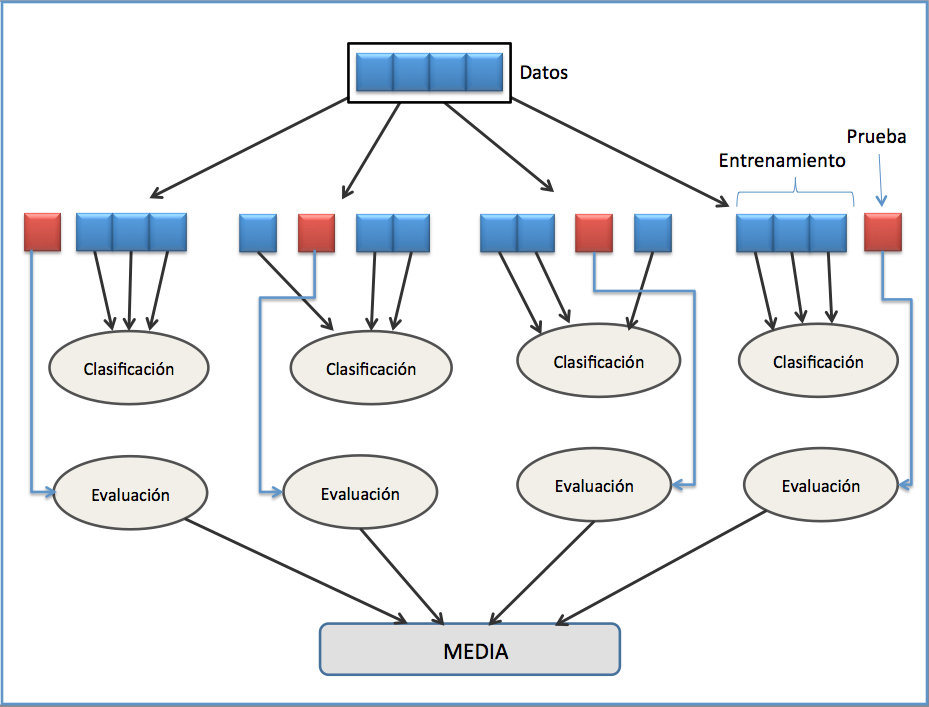
\includegraphics{cv.jpg}
    \end{center}
\end{frame}
\note{
    TODO: decir ventajas
}

% TODO: poner o no lo de subcorpus?

\subsection{Línea base}
\begin{frame}
    \frametitle{Línea base}

    Línea base
\end{frame}

\subsection{Características}
\begin{frame}
    \frametitle{Características}

    Características
\end{frame}

\subsection{Primer clasificador}
\begin{frame}
    \frametitle{Primer clasificador}

    Primer clasificador
\end{frame}

\subsection{Selección de características}
\begin{frame}
    \frametitle{Selección de características}

    Selección de características
\end{frame}

\subsection{Clasificador final}
\begin{frame}
    \frametitle{Clasificador final}

    Clasificador final
\end{frame}

\subsection{Otros análisis}
\begin{frame}
    \frametitle{Otros análisis}

    Otros análisis
\end{frame}
